\chapter{Teknologi}
\label{chap:teknologiafsnit}
\section{Indledning}

Videokonferencer giver i dag mulighed for, at sundhedsfagligt personale kan kommunikere med borgere på helt nye måder.
\\
Som konsekvens af den teknologiske udvikling opstår der nye problemstillinger, hvor bl.a. infrastruktur og patientsikkerhed er nøglebegreber, der sætter tekniske og lovmæssige krav til behandlingen og ikke mindst overførsel af data.
\\
I dette afsnit kigges der nærmere på Appinux, som leverer videokonferencesystemet til Favrskov Kommune, og det undersøges, hvorvidt denne løsning harmonerer med de nævnte forudsætninger og det diskuteres, hvilke andre teknologiske foranstaltninger en leverandør af sundhedsydelser som Favrskov Kommune bør være opmærksom på.

\subsection{Fokuseret spørgsmål}
\begin{itemize}
	\item Hvordan fungerer Appinux-løsningen med videoopkald i Favrskov Kommune? \\Spørgsmålet søges besvaret med udgangspunkt i følgende punkter:
	\begin{itemize}
	\item Sikkerhedskrav
	\item Dækning 
	\item Kompatibilitet 
\end{itemize}
\end{itemize}


\section{Metode}
Dette afsnit bygger på informationer fra møder og emailkorrespondencer med Appinux' salgdirektør, Michael Ellegaard. Det har været været vanskeligt at finde litteratur, der direkte undersøger Appinux' løsning, så fokus har i stedet ligget på de delelementer og standarder, som Appinux anvender og bygger på. Der er deraf foretaget litteratursøgning på dette med henblik på at klarlægge både mangler og muligheder af produktet inden for infrastruktur. Der er anvendt en kvalitativ undersøgelse i form af en struktureret interviewundersøgelse.

Specifikke emneord: \textit{WebRTC, Bandwidth.}

For en dybdegående beskrivelse af metoden henvises til afsnittet Metode 2. 



\section{Resultater}
Der er udarbejdet en oversigt over elementer, der bør tages med i betragtning i forbindelse med implementering af Appinux løsning. Dette ses i tabel\ref{tab:tabelforud}.
\begin{table}[H]
\caption{Oversigt over vigtige forudsætninger i forbindelse med implementeringen af Appinux' videomodul.}
\centering
\label{tab:tabelforud}
\begin{tabular}{|p{0.2\linewidth}m{0.5\linewidth}|}
\hline
\textbf{Forudsætninger} & \\ \hline
Infrastruktur & \begin{itemize}\item Båndbredde\item Dækning \end{itemize}\\ \hline
Sikkerhed & \begin{itemize}\item Lovkrav\item Kryptering \end{itemize}\\ \hline
Udstyr & \begin{itemize}\item Hardwarespecifikationer \item Styresystemsspecifikationer \item Opdateringer \item Support \end{itemize}\\ \hline
\end{tabular}

\end{table}
\subsection{Appinux}
Dette afsnit bygger på mødereferat med salgdirektør fra Appinux, Michael Ellegaard [Bilag 4, 4.1], samt Appinux' website \cite{appinuxwebsite}.\\Der er taget udgangspunkt i, at de givne informationer er korrekte, da det ikke har været muligt at finde relevant information om Appinux' løsning andetsteds.\\
Appinux er en multiplatformsløsning, der giver mulighed for at vælge og fravælge over 70 moduler efter den gågældende kundes behov. Appinux er platformsuafhængig i den forstand, at det kan køre på PC'er via Google Chrome, samt  smartphones og tablets, der er forsynet med Android v. 4.02.\\Der gives, udover Appinux' egne moduler, også adgang til, at tredjepartsfirmaer kan implementere deres egne moduler under forudsætning af, at der finder et samarbejde sted. Dette er for eksempel i form af et genoptræningsmodul.\\Videokonferencesystemet er Appinux' eget modul. Platformen fungerer ved, at Chrome åbnes på enten en PC eller via en app på en smartphone eller tablet, hvorved der er adgang til modulet, som anvender WebRTC. WebRTC er et open source-projekt, som giver mulighed for realtidskommunikation via en browser \cite{webrtchjemmeside}. Det har den funktion, at videokvaliteten bliver justeret efter tilgængelig båndbredde og CPU-kraft hos hhv. afsender og modtager. Det vurderes af Appinux, at en båndbredde på 512kbit/s er minimumskrav for at videokonferencesystemet kører flydende.

Appinux følger en række standarder, som er væsentlige   er nævne. \textit{Continua Health Alliance} giver mulighed for plug-and-play af diverse apparater, såsom en blodtrykmåler, hvilket øger tilslutningsmulighederne. Der gives dog udtryk for, at det primært sker gennem aftaler mellem Appinux og tredjepartsleverandører. Inden for integration understøttes \textit{HL7}, herunder også \textit{FHIR}, som er en standard der sikrer konsistent dataudvekling mellem medicinske systemer [Bilag 4, 4.1]. Derudover giver Appinux mulighed for at opsamle en række data om borgeren, som kan tilgås via grafer og eksporteres ud af systemet.

\subsection{Infrastruktur}
Telekommunikation som videokonferencesystemer er afhængig af tilstedeværelsen af en  internetforbindelse.\\
Overordnet set skelner denne mini-MTV mellem mobilt bredbånd og en kablet forbindelse, som inkluderer fiber-, coaxial- og kobberforbindelser, da det er her det største skel i forhold til videokonferencesystemer ligger.\\
Internethastigheden eller båndbredden er ofte den parameter, der kigges på, når kvaliteten på en internetopkobling vurderes. Den mest udbredte opkoblingstype i Danmark er ADSL-bredbånd med over en million abonnementer \cite{statadsl}. Hastighed på disse ligger typisk fra 10/1Mbit/s til 100/20Mbit/s \cite{tdchastigheder} \cite{telenorhastigheder}. Det har ikke været muligt at finde et dækningskort, der viser fiber- og bredbåndsdækningen i Favrskov Kommune, men denne mini-MTV tager udgangspunkt i, at hvis en borger har købt bredbånd med en given hastighed, bliver produktet også leveret.\\
Udover den kablede internetopkobling, er det også muligt at tilgå internettet via det mobile netværk. Eftersom det hele kører trådsløs, er dækningen utrolig vigtig for, at et videokonferencesystem kører optimalt. TDC's dækningskort viser, at Favrskov Kommune har min. 5Mbit/s på enten 3G- eller 4G-netværket udendørs \cite{tdcdaekning}.
%Det kan dog være svært at sige, hvorledes hastigheden stemmer overens indendørs, og det er dermed vigtigt at undersøge dette i hver given sitution.
Der har været indberetninger fra borgere, der antyder, at der i kommunen i efteråret 2015 var problemer med mobildækningen indendørs\cite{tv2oj_daekning}, hvilket har udmøntet sig i et dækningskort som vist på figur \ref{fig:dkort}. Dette indikerer, at kommunen er opmærksom på problemet.\\
Der arbejdes løbende på en forbedret dækning og bredbåndshastighed med en målsætning på 100Mbit/s download og 30Mbit/s upload til alle danskere i 2020\cite{digitalvel}.
\begin{figure}[H]
\centering
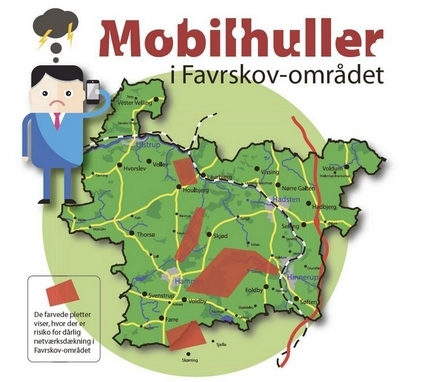
\includegraphics[width=0.7\textwidth]{Figurer/daekningskort.png}
\caption{\label{fig:dkort}Dækningskort for mobildækning i Favrskov Kommune fra sommer 2015. De røde pletter angiver områder med dårlig dækning [Bilag 14, 14.1]}
\end{figure}

\subsection{Sikkerhed}
Når patientfølsomme data sendes rundt i cyberspace, er der visse lovkrav, der skal sikre, at der i tilstrækkelig grad værnes om disse data.
Sundhedsstyrelsen udgav i 2008 \citetitle{vogi}, som omhandler ændringer i sundhedsloven vedrørende elektroniske systemer. Denne blev i 2015 revideret, og det er primært denne, der er anvendt som informationskilde \cite{vogi}.\\
Det bemærkes, at kilden er et høringsudkast, så ændringer må forventes at forekomme.\\
Offentlige institutioner inden for sundhedssektoren, der kommunikerer via internettet skal anvende en krypteret forbindelse, og brugeren skal anvende en såkaldt tofaktor-autentifikation, som består af en login-funktion, der både indeholder noget de ved og noget de har. Nem-ID er et eksempel herpå \cite{vogi}. Private er ikke underlagt samme restriktioner, men det anbefales, at der anvendes tilsvarende eller samme løsning.

Den dataansvarlige skal overholde sikkerhedsbekendtgørelsens krav, hvilket blandt andet indebærer, at det data, der lagres på enheden, skal være krypteret og beskyttet med kode og kommunikation mellem enhed og database skal være krypteret \cite{shbekendt}. Yderligere skal det sikres, at andre væsentlige forhold fra sundhedsloven, autorisationsloven samt persondataloven overholdes. 

\section{Diskussion}
\subsection{Appinux på netværket}
Med udgangspunkt i det foregående er der fundet evidens for, at den digitale infrastruktur i Favrskov Kommune i teorien er stærk nok til, at videokonferencesystemet fra Appinux kan køre stabilt. Eftersom videoløsningen selv kan justere kvaliteten på baggrund af internetforbindelsen, er systemet ikke så afhængig af stabilitet i båndbredden, men dækningen skal stadig være tilstrækkelig, hvilket kan volde problemer i nogle områder af kommunen.\\
%Det findes derfor nødvendigt at teste forbindelsen hos den enkelte borger, såfremt borgeren er nødsaget til at køre over det mobile netværk via et SIM-kort. Et andet problem med det mobile netværk er, at der kan opstå forsinkelse i samtalen.\\
Det er blevet konkluderet i studiet \citetitle{webrtcjournal}, der har undersøgt WebRTC på en 3G-forbindelse, at der kan være forsinkelse på op til næsten to sekunder, og dette bliver igen påvirket af flere parametre og giver ifølge studiet svingninger i forsinkelsestiden \cite{webrtcjournal}. Det bør dog nævnes, at 4G-dækning ikke er med i undersøgelsen. Desuden er undersøgelsen lavet i 2013, mens WebRTC stadig var i udviklingsfasen, så omstændighederne kan være anderledes, og en ny tilsvarende undersøgelse er relevant.

Det har ikke været muligt at finde videnskabelige artikler, der undersøger WebRTC på forskellige båndbredder, men videolink2.me er en leverandør af en tilsvarende løsning, der også anvender WebRTC, og denne leverandør har opsat en række minimumskrav og anbefalinger til båndbredden, som ses i tabel \ref{tab:hastighedtabel}. Disse stemmer godt overens med Appinux' anbefalinger [Bilag 4, 4.1].
\begin{table}[H]
\caption{Bud på hastighedskrav til internetopkoblingen ved brug af WebRTC lavet baseret på tabel af VideoLink2.me \cite{videolink2me}}
\label{tab:hastighedtabel}
\centering
\begin{tabular}{|l|l|l|}
\hline
\textbf{Antal brugere} & \textbf{Minimum} [kb/s]  & \textbf{Anbefalet}  [kb/s] \\ \hline
1             & 150          & 256          \\ \hline
2             & 300          & 512          \\ \hline
3             & 450          & 768          \\ \hline
4             & 600          & 1024          \\ \hline
5             & 750          & 1280          \\ \hline
\end{tabular}

\end{table}

\subsubsection{Struktureret interviewundersøgelse}
Udfordringerne med forsinkelsestid understøttes yderligere af interviewundersøgelsen fra \textit{Pilotprojekt Videokommunikation}, hvor to sygeplejersker angav, at der kunne være forsinkelse på lyd og billede afhængig af geografisk placering. \\Yderligere blev der rapporteret om billedudfald, samt at billedekvaliteten kunne forbedres [Bilag 7, 7.1]. I interviewundersøgelsen er der blevet spurgt fire borgere og to sygeplejesker, så generaliserbarheden kunne forbedres. Ligeledes bør konklusioner inden for disse områder drages på baggrund af mere tekniske undersøgelser af kvantitativ karakter.


\subsection{Opfyldning af sikkerhedskrav}
Anbefalingen om en tofaktor-autentifikation, der er pålagt offentlige institutioner at følge, anvendes ikke af Appinux. For at logge ind anvendes blot brugernavn og kodeord, og så er brugeren logget ind i en given periode. For at højne sikkerheden kunne borgeren logge ind med Nem-ID. Dette ville dog tidsmæssigt besværliggøre processen og muligvis være til gene. Teknologien, der muliggør Nem-ID på Android-systemer, findes og anvendes af blandt andre Nets \cite{netsapp}.\\
Samtaletidspunkt, varighed og opkalds-ID logges, men selve samtalen gemmes ikke. Det er derved ikke aktuelt at bedømme, hvorledes denne krypteres på enheden. Selve videokonferencen foregår via en sikker protokol i form af HTTPS [Bilag 4, 4.1].\\
Som udgangspunkt opfylder Appinux altså minimumskravene, men der gøres opmærksom på, at det er Favrskov Kommunes ansvar, at sikkerhedskrav samt lovgivning bliver overholdt. Desuden er det vigtigt ved eventuelle ændringer i lovgivningen, at kommunen sørger for, at Appinux opdateres.

\subsection{Implementeringsprocessen}
\label{sec:implementeringsprocessen}
Appinux lægger vægt på, at kommunen skal være selvhjulpne og blander sig nødigt i implementeringsfasen. Som konsekvens herpå stod kommunen med tablets, som ikke opfyldte minimumskravene til at køre Appinux, hvorfor de måtte erstattes af nye. I denne forbindelse havde det været fordelagtigt med nogle på forhånd klare minimumskrav til specifikationer til PC, tablet og smartphone fra Appinux' side.\\Disse kunne pr. efterspørgsel ikke opgives, hvilket stiller Favrskov Kommune i den situation, at de ikke ved, hvilket udstyr, der virker med Appinux. Det er ligeledes kommunens ansvar at undgå opdateringer af styresystemet på enheden, da Appinux ikke tager ansvar for, at app'en derefter stadig virker. Der bør derfor være en sikring i selve enheden, der sørger for, at dette ikke sker, da en nedgradering kan være vanskelig at udføre.
\subsection{Kompatabilitet}
Det anbefales også, at kommunen tester, at det er muligt at hive data ud af systemet, således at den ikke binder sig til Appinux på længere sigt. I og med at Appinux understøtter \textit{FHIR}-standarden, bør det være muligt at udveklse data mellem andre systemer, der understøtter standarden. Det vurderes, at Appinux er en åben platform og at det er simpelt at udvide med nye komponenter, hvilket gør systemet meget alsidigt. Appinux bygger på open source-komponenter og er et selverklæret open source-system. Det har dog pr. efterspørgsmål ikke været muligt at få adgang til kildekoden, så dette stilles der spørgsmålstegn ved.\\Open source giver mulighed for, at andre levenrandørere nemt kan lave et tilsvarende system og bygge oven på den eksisterende løsning. Er der mulighed for at anvende et open source-system, vil det være anbefalelsesværdigt.
\subsection{Konklusion}
I dette teknologiafsnit er det blevet undersøgt, hvorvidt Appinux’ produkt til videoopkald harmonerer med sikkerhedskrav og den digitale infrastruktur i form af mobildækning og bredbåndshastigheder i Favrskov Kommune.
Det konkluderes, at Appinux’ produkt til virtuel hjemmepleje kan erstatte eller supplere fysiske besøg på et acceptabelt billedkvalitet, såfremt dækning og båndbredde er tilstrækkelig.
\\Der er fra borgernes side indberettet dækningsproblemer, og Favrskov Kommune bør i den forbindelse undersøge dækningsforholdende inden løsningen implementeres hos den pågældende borger, da der ellers i følge studiet \citetitle{webrtcjournal} og den strukturerede interviewundersøgelse kan opstå forsinkelse og lav billedkvalitet.\\
Appinux overholder minimumskravene i forhold til datakryptering, da løsningen kører på en sikker protokol i form af HTTPS. Udover dette anvendes et login, som består af et brugernavn samt kodeord. For at forbedre sikkerheden anbefaler Sundhedsstyrelsen en tofaktor-autentifikation i form af Nem-ID eller lignende. Det er Favrskov Kommunes ansvar at beskytte patienters oplysninger i henhold til sundhedsloven.\\ 
Favrskov Kommune stod for at implementere løsningen, da Appinux ikke har et implementeringshold, som varetager denne opgave, der opstod i den forbindelse problemer på grund af mangel på minimumskrav fra Appinux' side. Det er yderligere vigtigt, at det på forhånd er undersøgt, hvorledes data kan hives ud af systemet, og hvorvidt der kan bygges videre på løsningen, så et eventuelt leverandørskifte forekommer så gnidningsfrit som muligt og uden datatab.
